\documentclass[11pt,letterpaper]{article}
\usepackage[utf8]{inputenc}
\usepackage[top=1in,bottom=1in,left=1in,right=1in]{geometry}
\usepackage{amsmath}
\usepackage{amsfonts}
\usepackage{amssymb}
\usepackage{amsthm}
\usepackage{bm}
\usepackage{braket}
\usepackage{cancel}
\usepackage{enumitem}
\usepackage{float}
\usepackage[T1]{fontenc}
\usepackage{forloop}
\usepackage{graphicx}
\usepackage{hyperref}
\usepackage{lmodern}
\usepackage{mathabx}
\usepackage{parskip}
\usepackage{subcaption}
\usepackage{tensor}
\usepackage{titlesec}
\usepackage{titling}
\usepackage{listings}

\lstset{basicstyle=\footnotesize\ttfamily}

\setenumerate{leftmargin=*}


% \titlelabel{(\thetitle)\quad}
\titleformat*{\section}{\large\bfseries}
\titleformat*{\subsection}{\normalsize\bfseries}
\setlength{\droptitle}{-5em}


\DeclareMathOperator*{\argmin}{arg\,min}
\DeclareMathOperator*{\argmax}{arg\,max}

\DeclareMathOperator{\tr}{tr}

\let\Re\relax
\DeclareMathOperator{\Re}{Re}
\let\Im\relax
\DeclareMathOperator{\Im}{Im}

\DeclareMathOperator{\sgn}{sgn}

\newcommand{\R}{\mathbb{R}}


\theoremstyle{definition}
\newtheorem{defn}{Definition}[section]

\theoremstyle{plain}
\newtheorem{thm}{Theorem}[section]



\newcommand{\bhat}[1]{\hat{\bm{#1}}}
\newcommand{\prop}{\mathrel{\propto}}


\renewcommand{\thesubsection}{\normalsize \alph{subsection}}
\renewcommand{\d}{\mathrm{d}}
\renewcommand{\vec}[1]{\bm{#1}}
\newcommand{\del}{\vec{\nabla}}
\newcommand{\e}{\epsilon}
\newcommand{\tpd}[3]{\left( \frac{\partial #1}{\partial #2} \right)_{#3}}
\newcommand{\pd}[2]{\frac{\partial #1}{\partial #2}}
\newcommand{\spd}[2]{\frac{\partial^2 #1}{\partial {#2}^2}}
\def\dbar{{\mathchar'26\mkern-12mu d}}

\allowdisplaybreaks


\author{Sam Kowash}
\numberwithin{equation}{section}
\numberwithin{figure}{section}
\title{CSE 546 HW \#3 Problem 5 Revisited}

\begin{document}
\maketitle


\section{Movie Recommender System}
\begin{enumerate}
\setcounter{enumi}{4}
	\item 	Based on a partial data set of $n=1000$ users rating in $[-10,10]$ a subset of $m=500$ movies, we estimate those users' ratings of unrated movies. We do this by developing $d$-dimensional vector models representing each user by a vector $u_i$ and each movie by a vector $v_j$, then estimating user $i$'s rating of movie $j$ by $\langle u_i, v_j \rangle$.
	\begin{enumerate}
		\item First, we try the most naive approach and simply complete each empty entry in each column $j$ with the average user's rating of movie $j$. This achieves a mean squared training error of $0.559$ and a mean absolute training error of $0.596$. The squared and absolute \emph{test} errors (from users' additional held-out ratings) were $0.570$ and $0.602$, respectively.

		\item Next, we suppose all omitted ratings are zero and generate vector representations with $\{u_i\}$ and $\{v_j\}$ as the first $d$ left- and right-singular vectors of the data matrix, respectively (with the singular value matrix multiplied into $V^T$). Squared and absolute train and test errors shown in Fig.~\ref{fig:svd}.

		\begin{figure}[H]
			\centering
			\begin{subfigure}[t]{0.48\textwidth}
			\centering
			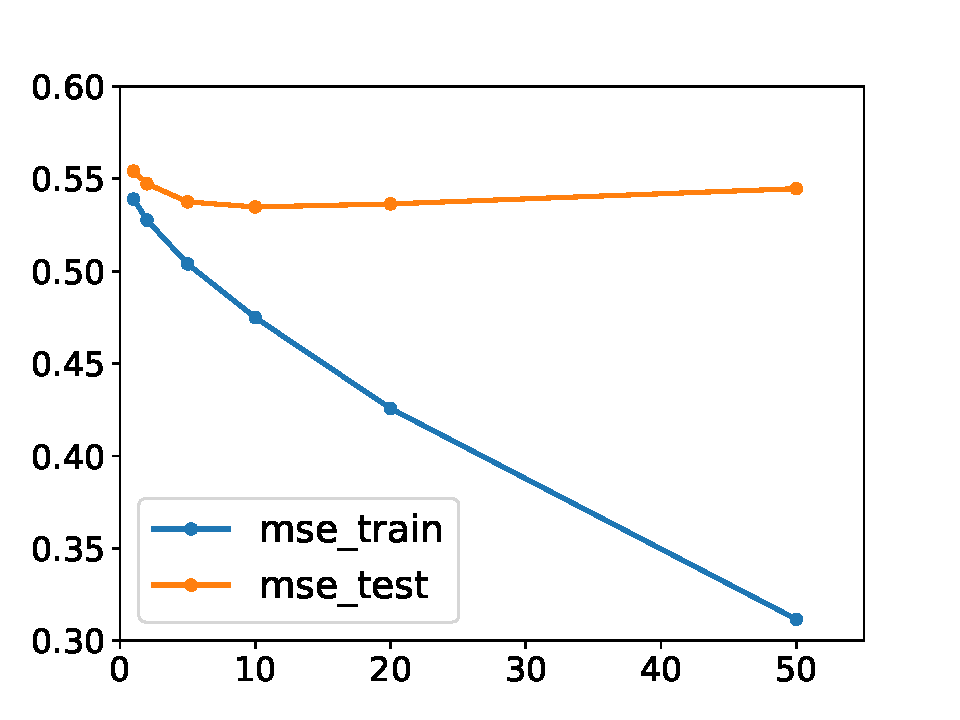
\includegraphics[width=\textwidth]{figures/svd_mse.pdf}
			\caption{MSEs for SVD representations at different $d$}
			\end{subfigure}
			%
			\begin{subfigure}[t]{0.48\textwidth}
			\centering
			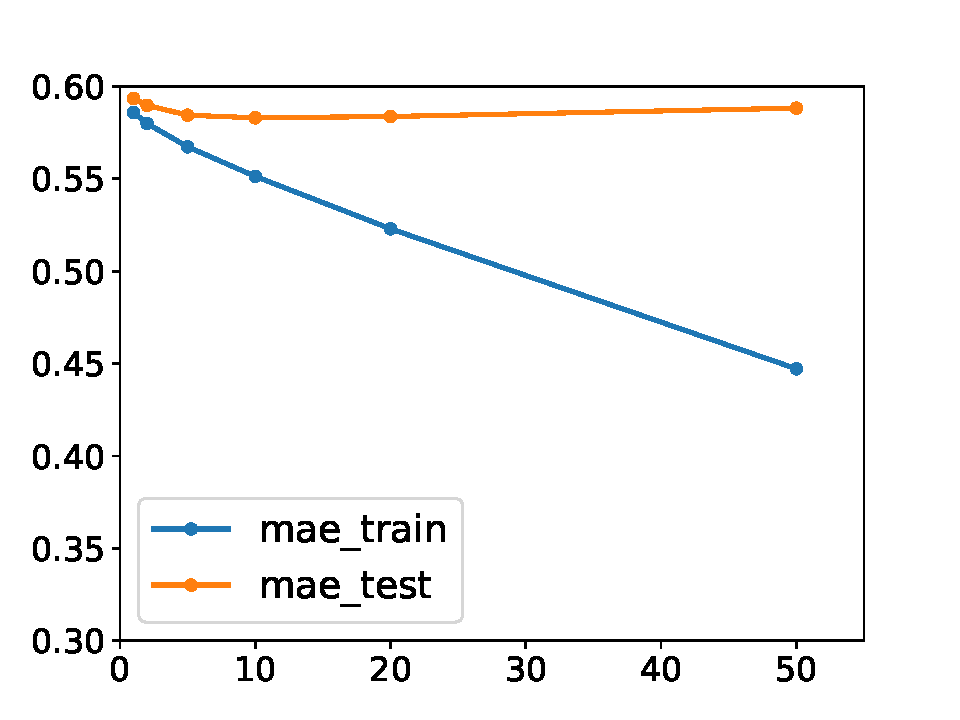
\includegraphics[width=\textwidth]{figures/svd_mae.pdf}
			\caption{MAEs for SVD representations at different $d$}
			\end{subfigure}
			\caption{}\label{fig:svd}
		\end{figure}


		\item Lastly, we try to improve on these results by minimizing an objective which only accumulates error over extant ratings, rather than substituting values.
		%
		\begin{align*}
			L\left(\{u_i\},\{v_j\}\right) &= \sum_{(i,j)\in T} \left(\braket{u_i,v_j} - R_{ij}\right)^2 + \lambda \sum_{i=1}^n \|u_i\|_2^2 + \lambda \sum_{j=1}^m \|v_j\|_2^2
		\end{align*}
		%
		Here $\lambda$ is a regularization hyperparameter to constrain the vector magnitudes. We can approach this through alternating minimization, where if we fix $\{v_i\}$ we can see that each $u_i$ should become
		%
		\begin{align*}
			\hat{u}_i &= \left(\sum_j v_j v_j^T + \lambda I\right)^{-1} \left(\sum_j R_{ij} v_j\right),
		\end{align*}
		%
		and each $v_j$ should be updated by an exactly symmetric expression. Unfortunately, code still has bugs (dimension mismatch I haven't found yet) and I have no result for this part.
	\end{enumerate}
\end{enumerate}













\clearpage
\lstinputlisting[language=Python]{code/movie_recommend.py}
\end{document}